% Created by tikzDevice version 0.6.2-92-0ad2792 on 2013-03-23 22:56:34
% !TEX encoding = UTF-8 Unicode
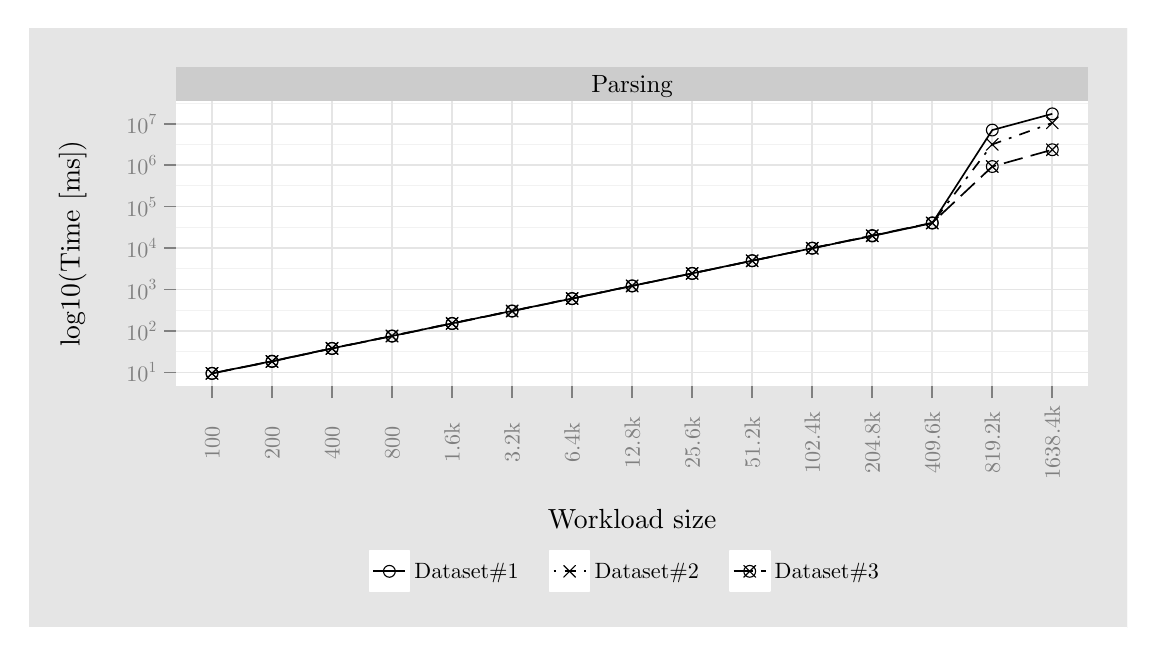
\begin{tikzpicture}[x=1pt,y=1pt]
\definecolor[named]{fillColor}{rgb}{1.00,1.00,1.00}
\path[use as bounding box,fill=fillColor,fill opacity=0.00] (0,0) rectangle (397.48,216.81);
\begin{scope}
\path[clip] (  0.00,  0.00) rectangle (397.48,216.81);
\definecolor[named]{drawColor}{rgb}{1.00,1.00,1.00}
\definecolor[named]{fillColor}{rgb}{0.90,0.90,0.90}

\path[draw=drawColor,line width= 0.6pt,line join=round,line cap=round,fill=fillColor] (  0.00,  0.00) rectangle (397.48,216.81);
\end{scope}
\begin{scope}
\path[clip] ( 53.58, 87.19) rectangle (383.26,190.36);
\definecolor[named]{fillColor}{rgb}{1.00,1.00,1.00}

\path[fill=fillColor] ( 53.58, 87.19) rectangle (383.26,190.36);
\definecolor[named]{drawColor}{rgb}{0.95,0.95,0.95}

\path[draw=drawColor,line width= 0.3pt,line join=round] ( 53.58, 99.73) --
	(383.26, 99.73);

\path[draw=drawColor,line width= 0.3pt,line join=round] ( 53.58,114.70) --
	(383.26,114.70);

\path[draw=drawColor,line width= 0.3pt,line join=round] ( 53.58,129.68) --
	(383.26,129.68);

\path[draw=drawColor,line width= 0.3pt,line join=round] ( 53.58,144.66) --
	(383.26,144.66);

\path[draw=drawColor,line width= 0.3pt,line join=round] ( 53.58,159.63) --
	(383.26,159.63);

\path[draw=drawColor,line width= 0.3pt,line join=round] ( 53.58,174.61) --
	(383.26,174.61);

\path[draw=drawColor,line width= 0.3pt,line join=round] ( 53.58,189.58) --
	(383.26,189.58);
\definecolor[named]{drawColor}{rgb}{0.90,0.90,0.90}

\path[draw=drawColor,line width= 0.6pt,line join=round] ( 53.58, 92.24) --
	(383.26, 92.24);

\path[draw=drawColor,line width= 0.6pt,line join=round] ( 53.58,107.22) --
	(383.26,107.22);

\path[draw=drawColor,line width= 0.6pt,line join=round] ( 53.58,122.19) --
	(383.26,122.19);

\path[draw=drawColor,line width= 0.6pt,line join=round] ( 53.58,137.17) --
	(383.26,137.17);

\path[draw=drawColor,line width= 0.6pt,line join=round] ( 53.58,152.14) --
	(383.26,152.14);

\path[draw=drawColor,line width= 0.6pt,line join=round] ( 53.58,167.12) --
	(383.26,167.12);

\path[draw=drawColor,line width= 0.6pt,line join=round] ( 53.58,182.09) --
	(383.26,182.09);

\path[draw=drawColor,line width= 0.6pt,line join=round] ( 66.60, 87.19) --
	( 66.60,190.36);

\path[draw=drawColor,line width= 0.6pt,line join=round] ( 88.29, 87.19) --
	( 88.29,190.36);

\path[draw=drawColor,line width= 0.6pt,line join=round] (109.97, 87.19) --
	(109.97,190.36);

\path[draw=drawColor,line width= 0.6pt,line join=round] (131.66, 87.19) --
	(131.66,190.36);

\path[draw=drawColor,line width= 0.6pt,line join=round] (153.35, 87.19) --
	(153.35,190.36);

\path[draw=drawColor,line width= 0.6pt,line join=round] (175.04, 87.19) --
	(175.04,190.36);

\path[draw=drawColor,line width= 0.6pt,line join=round] (196.73, 87.19) --
	(196.73,190.36);

\path[draw=drawColor,line width= 0.6pt,line join=round] (218.42, 87.19) --
	(218.42,190.36);

\path[draw=drawColor,line width= 0.6pt,line join=round] (240.11, 87.19) --
	(240.11,190.36);

\path[draw=drawColor,line width= 0.6pt,line join=round] (261.80, 87.19) --
	(261.80,190.36);

\path[draw=drawColor,line width= 0.6pt,line join=round] (283.49, 87.19) --
	(283.49,190.36);

\path[draw=drawColor,line width= 0.6pt,line join=round] (305.18, 87.19) --
	(305.18,190.36);

\path[draw=drawColor,line width= 0.6pt,line join=round] (326.87, 87.19) --
	(326.87,190.36);

\path[draw=drawColor,line width= 0.6pt,line join=round] (348.56, 87.19) --
	(348.56,190.36);

\path[draw=drawColor,line width= 0.6pt,line join=round] (370.25, 87.19) --
	(370.25,190.36);
\definecolor[named]{drawColor}{rgb}{0.00,0.00,0.00}

\path[draw=drawColor,line width= 0.6pt,line join=round] ( 66.60, 91.90) --
	( 88.29, 96.31) --
	(109.97,100.92) --
	(131.66,105.40) --
	(153.35,109.96) --
	(175.04,114.45) --
	(196.73,118.90) --
	(218.42,123.50) --
	(240.11,128.03) --
	(261.80,132.61) --
	(283.49,137.11) --
	(305.18,141.53) --
	(326.87,146.18) --
	(348.56,179.81) --
	(370.25,185.67);

\path[draw=drawColor,line width= 0.6pt,dash pattern=on 1pt off 3pt on 4pt off 3pt ,line join=round] ( 66.60, 91.92) --
	( 88.29, 96.24) --
	(109.97,100.96) --
	(131.66,105.43) --
	(153.35,110.01) --
	(175.04,114.46) --
	(196.73,119.01) --
	(218.42,123.52) --
	(240.11,128.04) --
	(261.80,132.55) --
	(283.49,137.08) --
	(305.18,141.60) --
	(326.87,146.18) --
	(348.56,174.62) --
	(370.25,182.39);

\path[draw=drawColor,line width= 0.6pt,dash pattern=on 7pt off 3pt ,line join=round] ( 66.60, 91.88) --
	( 88.29, 96.18) --
	(109.97,100.87) --
	(131.66,105.34) --
	(153.35,109.88) --
	(175.04,114.38) --
	(196.73,118.90) --
	(218.42,123.48) --
	(240.11,127.99) --
	(261.80,132.58) --
	(283.49,137.14) --
	(305.18,141.69) --
	(326.87,146.30) --
	(348.56,166.63) --
	(370.25,172.70);

\path[draw=drawColor,line width= 0.4pt,line join=round,line cap=round] ( 66.60, 91.90) circle (  2.13);

\path[draw=drawColor,line width= 0.4pt,line join=round,line cap=round] ( 88.29, 96.31) circle (  2.13);

\path[draw=drawColor,line width= 0.4pt,line join=round,line cap=round] (109.97,100.92) circle (  2.13);

\path[draw=drawColor,line width= 0.4pt,line join=round,line cap=round] (131.66,105.40) circle (  2.13);

\path[draw=drawColor,line width= 0.4pt,line join=round,line cap=round] (153.35,109.96) circle (  2.13);

\path[draw=drawColor,line width= 0.4pt,line join=round,line cap=round] (175.04,114.45) circle (  2.13);

\path[draw=drawColor,line width= 0.4pt,line join=round,line cap=round] (196.73,118.90) circle (  2.13);

\path[draw=drawColor,line width= 0.4pt,line join=round,line cap=round] (218.42,123.50) circle (  2.13);

\path[draw=drawColor,line width= 0.4pt,line join=round,line cap=round] (240.11,128.03) circle (  2.13);

\path[draw=drawColor,line width= 0.4pt,line join=round,line cap=round] (261.80,132.61) circle (  2.13);

\path[draw=drawColor,line width= 0.4pt,line join=round,line cap=round] (283.49,137.11) circle (  2.13);

\path[draw=drawColor,line width= 0.4pt,line join=round,line cap=round] (305.18,141.53) circle (  2.13);

\path[draw=drawColor,line width= 0.4pt,line join=round,line cap=round] (326.87,146.18) circle (  2.13);

\path[draw=drawColor,line width= 0.4pt,line join=round,line cap=round] (348.56,179.81) circle (  2.13);

\path[draw=drawColor,line width= 0.4pt,line join=round,line cap=round] (370.25,185.67) circle (  2.13);

\path[draw=drawColor,line width= 0.4pt,line join=round,line cap=round] ( 64.46, 89.78) -- ( 68.73, 94.05);

\path[draw=drawColor,line width= 0.4pt,line join=round,line cap=round] ( 64.46, 94.05) -- ( 68.73, 89.78);

\path[draw=drawColor,line width= 0.4pt,line join=round,line cap=round] ( 86.15, 94.11) -- ( 90.42, 98.38);

\path[draw=drawColor,line width= 0.4pt,line join=round,line cap=round] ( 86.15, 98.38) -- ( 90.42, 94.11);

\path[draw=drawColor,line width= 0.4pt,line join=round,line cap=round] (107.84, 98.83) -- (112.11,103.10);

\path[draw=drawColor,line width= 0.4pt,line join=round,line cap=round] (107.84,103.10) -- (112.11, 98.83);

\path[draw=drawColor,line width= 0.4pt,line join=round,line cap=round] (129.53,103.30) -- (133.80,107.56);

\path[draw=drawColor,line width= 0.4pt,line join=round,line cap=round] (129.53,107.56) -- (133.80,103.30);

\path[draw=drawColor,line width= 0.4pt,line join=round,line cap=round] (151.22,107.88) -- (155.49,112.14);

\path[draw=drawColor,line width= 0.4pt,line join=round,line cap=round] (151.22,112.14) -- (155.49,107.88);

\path[draw=drawColor,line width= 0.4pt,line join=round,line cap=round] (172.91,112.32) -- (177.18,116.59);

\path[draw=drawColor,line width= 0.4pt,line join=round,line cap=round] (172.91,116.59) -- (177.18,112.32);

\path[draw=drawColor,line width= 0.4pt,line join=round,line cap=round] (194.60,116.87) -- (198.87,121.14);

\path[draw=drawColor,line width= 0.4pt,line join=round,line cap=round] (194.60,121.14) -- (198.87,116.87);

\path[draw=drawColor,line width= 0.4pt,line join=round,line cap=round] (216.29,121.39) -- (220.55,125.66);

\path[draw=drawColor,line width= 0.4pt,line join=round,line cap=round] (216.29,125.66) -- (220.55,121.39);

\path[draw=drawColor,line width= 0.4pt,line join=round,line cap=round] (237.98,125.90) -- (242.24,130.17);

\path[draw=drawColor,line width= 0.4pt,line join=round,line cap=round] (237.98,130.17) -- (242.24,125.90);

\path[draw=drawColor,line width= 0.4pt,line join=round,line cap=round] (259.67,130.41) -- (263.93,134.68);

\path[draw=drawColor,line width= 0.4pt,line join=round,line cap=round] (259.67,134.68) -- (263.93,130.41);

\path[draw=drawColor,line width= 0.4pt,line join=round,line cap=round] (281.35,134.95) -- (285.62,139.21);

\path[draw=drawColor,line width= 0.4pt,line join=round,line cap=round] (281.35,139.21) -- (285.62,134.95);

\path[draw=drawColor,line width= 0.4pt,line join=round,line cap=round] (303.04,139.46) -- (307.31,143.73);

\path[draw=drawColor,line width= 0.4pt,line join=round,line cap=round] (303.04,143.73) -- (307.31,139.46);

\path[draw=drawColor,line width= 0.4pt,line join=round,line cap=round] (324.73,144.04) -- (329.00,148.31);

\path[draw=drawColor,line width= 0.4pt,line join=round,line cap=round] (324.73,148.31) -- (329.00,144.04);

\path[draw=drawColor,line width= 0.4pt,line join=round,line cap=round] (346.42,172.48) -- (350.69,176.75);

\path[draw=drawColor,line width= 0.4pt,line join=round,line cap=round] (346.42,176.75) -- (350.69,172.48);

\path[draw=drawColor,line width= 0.4pt,line join=round,line cap=round] (368.11,180.26) -- (372.38,184.52);

\path[draw=drawColor,line width= 0.4pt,line join=round,line cap=round] (368.11,184.52) -- (372.38,180.26);

\path[draw=drawColor,line width= 0.4pt,line join=round,line cap=round] ( 66.60, 91.88) circle (  2.13);

\path[draw=drawColor,line width= 0.4pt,line join=round,line cap=round] ( 64.46, 89.74) -- ( 68.73, 94.01);

\path[draw=drawColor,line width= 0.4pt,line join=round,line cap=round] ( 64.46, 94.01) -- ( 68.73, 89.74);

\path[draw=drawColor,line width= 0.4pt,line join=round,line cap=round] ( 88.29, 96.18) circle (  2.13);

\path[draw=drawColor,line width= 0.4pt,line join=round,line cap=round] ( 86.15, 94.05) -- ( 90.42, 98.31);

\path[draw=drawColor,line width= 0.4pt,line join=round,line cap=round] ( 86.15, 98.31) -- ( 90.42, 94.05);

\path[draw=drawColor,line width= 0.4pt,line join=round,line cap=round] (109.97,100.87) circle (  2.13);

\path[draw=drawColor,line width= 0.4pt,line join=round,line cap=round] (107.84, 98.73) -- (112.11,103.00);

\path[draw=drawColor,line width= 0.4pt,line join=round,line cap=round] (107.84,103.00) -- (112.11, 98.73);

\path[draw=drawColor,line width= 0.4pt,line join=round,line cap=round] (131.66,105.34) circle (  2.13);

\path[draw=drawColor,line width= 0.4pt,line join=round,line cap=round] (129.53,103.20) -- (133.80,107.47);

\path[draw=drawColor,line width= 0.4pt,line join=round,line cap=round] (129.53,107.47) -- (133.80,103.20);

\path[draw=drawColor,line width= 0.4pt,line join=round,line cap=round] (153.35,109.88) circle (  2.13);

\path[draw=drawColor,line width= 0.4pt,line join=round,line cap=round] (151.22,107.75) -- (155.49,112.02);

\path[draw=drawColor,line width= 0.4pt,line join=round,line cap=round] (151.22,112.02) -- (155.49,107.75);

\path[draw=drawColor,line width= 0.4pt,line join=round,line cap=round] (175.04,114.38) circle (  2.13);

\path[draw=drawColor,line width= 0.4pt,line join=round,line cap=round] (172.91,112.24) -- (177.18,116.51);

\path[draw=drawColor,line width= 0.4pt,line join=round,line cap=round] (172.91,116.51) -- (177.18,112.24);

\path[draw=drawColor,line width= 0.4pt,line join=round,line cap=round] (196.73,118.90) circle (  2.13);

\path[draw=drawColor,line width= 0.4pt,line join=round,line cap=round] (194.60,116.76) -- (198.87,121.03);

\path[draw=drawColor,line width= 0.4pt,line join=round,line cap=round] (194.60,121.03) -- (198.87,116.76);

\path[draw=drawColor,line width= 0.4pt,line join=round,line cap=round] (218.42,123.48) circle (  2.13);

\path[draw=drawColor,line width= 0.4pt,line join=round,line cap=round] (216.29,121.34) -- (220.55,125.61);

\path[draw=drawColor,line width= 0.4pt,line join=round,line cap=round] (216.29,125.61) -- (220.55,121.34);

\path[draw=drawColor,line width= 0.4pt,line join=round,line cap=round] (240.11,127.99) circle (  2.13);

\path[draw=drawColor,line width= 0.4pt,line join=round,line cap=round] (237.98,125.86) -- (242.24,130.13);

\path[draw=drawColor,line width= 0.4pt,line join=round,line cap=round] (237.98,130.13) -- (242.24,125.86);

\path[draw=drawColor,line width= 0.4pt,line join=round,line cap=round] (261.80,132.58) circle (  2.13);

\path[draw=drawColor,line width= 0.4pt,line join=round,line cap=round] (259.67,130.44) -- (263.93,134.71);

\path[draw=drawColor,line width= 0.4pt,line join=round,line cap=round] (259.67,134.71) -- (263.93,130.44);

\path[draw=drawColor,line width= 0.4pt,line join=round,line cap=round] (283.49,137.14) circle (  2.13);

\path[draw=drawColor,line width= 0.4pt,line join=round,line cap=round] (281.35,135.01) -- (285.62,139.27);

\path[draw=drawColor,line width= 0.4pt,line join=round,line cap=round] (281.35,139.27) -- (285.62,135.01);

\path[draw=drawColor,line width= 0.4pt,line join=round,line cap=round] (305.18,141.69) circle (  2.13);

\path[draw=drawColor,line width= 0.4pt,line join=round,line cap=round] (303.04,139.56) -- (307.31,143.82);

\path[draw=drawColor,line width= 0.4pt,line join=round,line cap=round] (303.04,143.82) -- (307.31,139.56);

\path[draw=drawColor,line width= 0.4pt,line join=round,line cap=round] (326.87,146.30) circle (  2.13);

\path[draw=drawColor,line width= 0.4pt,line join=round,line cap=round] (324.73,144.16) -- (329.00,148.43);

\path[draw=drawColor,line width= 0.4pt,line join=round,line cap=round] (324.73,148.43) -- (329.00,144.16);

\path[draw=drawColor,line width= 0.4pt,line join=round,line cap=round] (348.56,166.63) circle (  2.13);

\path[draw=drawColor,line width= 0.4pt,line join=round,line cap=round] (346.42,164.49) -- (350.69,168.76);

\path[draw=drawColor,line width= 0.4pt,line join=round,line cap=round] (346.42,168.76) -- (350.69,164.49);

\path[draw=drawColor,line width= 0.4pt,line join=round,line cap=round] (370.25,172.70) circle (  2.13);

\path[draw=drawColor,line width= 0.4pt,line join=round,line cap=round] (368.11,170.57) -- (372.38,174.84);

\path[draw=drawColor,line width= 0.4pt,line join=round,line cap=round] (368.11,174.84) -- (372.38,170.57);
\end{scope}
\begin{scope}
\path[clip] (  0.00,  0.00) rectangle (397.48,216.81);
\definecolor[named]{fillColor}{rgb}{0.80,0.80,0.80}

\path[fill=fillColor] ( 53.58,190.36) rectangle (383.26,202.58);
\definecolor[named]{drawColor}{rgb}{0.00,0.00,0.00}

\node[text=drawColor,anchor=base,inner sep=0pt, outer sep=0pt, scale=  0.90] at (218.42,193.37) {Parsing};
\end{scope}
\begin{scope}
\path[clip] (  0.00,  0.00) rectangle (397.48,216.81);
\definecolor[named]{drawColor}{rgb}{0.50,0.50,0.50}

\node[text=drawColor,anchor=base west,inner sep=0pt, outer sep=0pt, scale=  0.80] at ( 35.67, 88.81) {10};

\node[text=drawColor,anchor=base west,inner sep=0pt, outer sep=0pt, scale=  0.56] at ( 43.67, 92.08) {1};

\node[text=drawColor,anchor=base west,inner sep=0pt, outer sep=0pt, scale=  0.80] at ( 35.67,103.78) {10};

\node[text=drawColor,anchor=base west,inner sep=0pt, outer sep=0pt, scale=  0.56] at ( 43.67,107.05) {2};

\node[text=drawColor,anchor=base west,inner sep=0pt, outer sep=0pt, scale=  0.80] at ( 35.67,118.76) {10};

\node[text=drawColor,anchor=base west,inner sep=0pt, outer sep=0pt, scale=  0.56] at ( 43.67,122.03) {3};

\node[text=drawColor,anchor=base west,inner sep=0pt, outer sep=0pt, scale=  0.80] at ( 35.67,133.74) {10};

\node[text=drawColor,anchor=base west,inner sep=0pt, outer sep=0pt, scale=  0.56] at ( 43.67,137.01) {4};

\node[text=drawColor,anchor=base west,inner sep=0pt, outer sep=0pt, scale=  0.80] at ( 35.67,148.71) {10};

\node[text=drawColor,anchor=base west,inner sep=0pt, outer sep=0pt, scale=  0.56] at ( 43.67,151.98) {5};

\node[text=drawColor,anchor=base west,inner sep=0pt, outer sep=0pt, scale=  0.80] at ( 35.67,163.69) {10};

\node[text=drawColor,anchor=base west,inner sep=0pt, outer sep=0pt, scale=  0.56] at ( 43.67,166.96) {6};

\node[text=drawColor,anchor=base west,inner sep=0pt, outer sep=0pt, scale=  0.80] at ( 35.67,178.66) {10};

\node[text=drawColor,anchor=base west,inner sep=0pt, outer sep=0pt, scale=  0.56] at ( 43.67,181.93) {7};
\end{scope}
\begin{scope}
\path[clip] (  0.00,  0.00) rectangle (397.48,216.81);
\definecolor[named]{drawColor}{rgb}{0.50,0.50,0.50}

\path[draw=drawColor,line width= 0.6pt,line join=round] ( 49.31, 92.24) --
	( 53.58, 92.24);

\path[draw=drawColor,line width= 0.6pt,line join=round] ( 49.31,107.22) --
	( 53.58,107.22);

\path[draw=drawColor,line width= 0.6pt,line join=round] ( 49.31,122.19) --
	( 53.58,122.19);

\path[draw=drawColor,line width= 0.6pt,line join=round] ( 49.31,137.17) --
	( 53.58,137.17);

\path[draw=drawColor,line width= 0.6pt,line join=round] ( 49.31,152.14) --
	( 53.58,152.14);

\path[draw=drawColor,line width= 0.6pt,line join=round] ( 49.31,167.12) --
	( 53.58,167.12);

\path[draw=drawColor,line width= 0.6pt,line join=round] ( 49.31,182.09) --
	( 53.58,182.09);
\end{scope}
\begin{scope}
\path[clip] (  0.00,  0.00) rectangle (397.48,216.81);
\definecolor[named]{drawColor}{rgb}{0.50,0.50,0.50}

\path[draw=drawColor,line width= 0.6pt,line join=round] ( 66.60, 82.92) --
	( 66.60, 87.19);

\path[draw=drawColor,line width= 0.6pt,line join=round] ( 88.29, 82.92) --
	( 88.29, 87.19);

\path[draw=drawColor,line width= 0.6pt,line join=round] (109.97, 82.92) --
	(109.97, 87.19);

\path[draw=drawColor,line width= 0.6pt,line join=round] (131.66, 82.92) --
	(131.66, 87.19);

\path[draw=drawColor,line width= 0.6pt,line join=round] (153.35, 82.92) --
	(153.35, 87.19);

\path[draw=drawColor,line width= 0.6pt,line join=round] (175.04, 82.92) --
	(175.04, 87.19);

\path[draw=drawColor,line width= 0.6pt,line join=round] (196.73, 82.92) --
	(196.73, 87.19);

\path[draw=drawColor,line width= 0.6pt,line join=round] (218.42, 82.92) --
	(218.42, 87.19);

\path[draw=drawColor,line width= 0.6pt,line join=round] (240.11, 82.92) --
	(240.11, 87.19);

\path[draw=drawColor,line width= 0.6pt,line join=round] (261.80, 82.92) --
	(261.80, 87.19);

\path[draw=drawColor,line width= 0.6pt,line join=round] (283.49, 82.92) --
	(283.49, 87.19);

\path[draw=drawColor,line width= 0.6pt,line join=round] (305.18, 82.92) --
	(305.18, 87.19);

\path[draw=drawColor,line width= 0.6pt,line join=round] (326.87, 82.92) --
	(326.87, 87.19);

\path[draw=drawColor,line width= 0.6pt,line join=round] (348.56, 82.92) --
	(348.56, 87.19);

\path[draw=drawColor,line width= 0.6pt,line join=round] (370.25, 82.92) --
	(370.25, 87.19);
\end{scope}
\begin{scope}
\path[clip] (  0.00,  0.00) rectangle (397.48,216.81);
\definecolor[named]{drawColor}{rgb}{0.50,0.50,0.50}

\node[text=drawColor,rotate= 90.00,anchor=base,inner sep=0pt, outer sep=0pt, scale=  0.80] at ( 69.35, 66.85) {100};

\node[text=drawColor,rotate= 90.00,anchor=base,inner sep=0pt, outer sep=0pt, scale=  0.80] at ( 91.04, 66.85) {200};

\node[text=drawColor,rotate= 90.00,anchor=base,inner sep=0pt, outer sep=0pt, scale=  0.80] at (112.73, 66.85) {400};

\node[text=drawColor,rotate= 90.00,anchor=base,inner sep=0pt, outer sep=0pt, scale=  0.80] at (134.42, 66.85) {800};

\node[text=drawColor,rotate= 90.00,anchor=base,inner sep=0pt, outer sep=0pt, scale=  0.80] at (156.11, 66.85) {1.6k};

\node[text=drawColor,rotate= 90.00,anchor=base,inner sep=0pt, outer sep=0pt, scale=  0.80] at (177.80, 66.85) {3.2k};

\node[text=drawColor,rotate= 90.00,anchor=base,inner sep=0pt, outer sep=0pt, scale=  0.80] at (199.49, 66.85) {6.4k};

\node[text=drawColor,rotate= 90.00,anchor=base,inner sep=0pt, outer sep=0pt, scale=  0.80] at (221.18, 66.85) {12.8k};

\node[text=drawColor,rotate= 90.00,anchor=base,inner sep=0pt, outer sep=0pt, scale=  0.80] at (242.86, 66.85) {25.6k};

\node[text=drawColor,rotate= 90.00,anchor=base,inner sep=0pt, outer sep=0pt, scale=  0.80] at (264.55, 66.85) {51.2k};

\node[text=drawColor,rotate= 90.00,anchor=base,inner sep=0pt, outer sep=0pt, scale=  0.80] at (286.24, 66.85) {102.4k};

\node[text=drawColor,rotate= 90.00,anchor=base,inner sep=0pt, outer sep=0pt, scale=  0.80] at (307.93, 66.85) {204.8k};

\node[text=drawColor,rotate= 90.00,anchor=base,inner sep=0pt, outer sep=0pt, scale=  0.80] at (329.62, 66.85) {409.6k};

\node[text=drawColor,rotate= 90.00,anchor=base,inner sep=0pt, outer sep=0pt, scale=  0.80] at (351.31, 66.85) {819.2k};

\node[text=drawColor,rotate= 90.00,anchor=base,inner sep=0pt, outer sep=0pt, scale=  0.80] at (373.00, 66.85) {1638.4k};
\end{scope}
\begin{scope}
\path[clip] (  0.00,  0.00) rectangle (397.48,216.81);
\definecolor[named]{drawColor}{rgb}{0.00,0.00,0.00}

\node[text=drawColor,anchor=base,inner sep=0pt, outer sep=0pt, scale=  1.00] at (218.42, 35.91) {Workload size};
\end{scope}
\begin{scope}
\path[clip] (  0.00,  0.00) rectangle (397.48,216.81);
\definecolor[named]{drawColor}{rgb}{0.00,0.00,0.00}

\node[text=drawColor,rotate= 90.00,anchor=base,inner sep=0pt, outer sep=0pt, scale=  1.00] at ( 18.80,138.77) {log10(Time [ms])};
\end{scope}
\begin{scope}
\path[clip] (  0.00,  0.00) rectangle (397.48,216.81);
\definecolor[named]{fillColor}{rgb}{0.90,0.90,0.90}

\path[fill=fillColor] (115.60,  8.87) rectangle (321.24, 31.86);
\end{scope}
\begin{scope}
\path[clip] (  0.00,  0.00) rectangle (397.48,216.81);
\definecolor[named]{drawColor}{rgb}{1.00,1.00,1.00}
\definecolor[named]{fillColor}{rgb}{1.00,1.00,1.00}

\path[draw=drawColor,line width= 0.6pt,line join=round,line cap=round,fill=fillColor] (123.48, 13.14) rectangle (137.93, 27.59);
\end{scope}
\begin{scope}
\path[clip] (  0.00,  0.00) rectangle (397.48,216.81);
\definecolor[named]{drawColor}{rgb}{0.00,0.00,0.00}

\path[draw=drawColor,line width= 0.6pt,line join=round] (124.92, 20.36) -- (136.49, 20.36);
\end{scope}
\begin{scope}
\path[clip] (  0.00,  0.00) rectangle (397.48,216.81);
\definecolor[named]{drawColor}{rgb}{0.00,0.00,0.00}

\path[draw=drawColor,line width= 0.4pt,line join=round,line cap=round] (130.70, 20.36) circle (  2.13);
\end{scope}
\begin{scope}
\path[clip] (  0.00,  0.00) rectangle (397.48,216.81);
\definecolor[named]{drawColor}{rgb}{1.00,1.00,1.00}
\definecolor[named]{fillColor}{rgb}{1.00,1.00,1.00}

\path[draw=drawColor,line width= 0.6pt,line join=round,line cap=round,fill=fillColor] (188.58, 13.14) rectangle (203.03, 27.59);
\end{scope}
\begin{scope}
\path[clip] (  0.00,  0.00) rectangle (397.48,216.81);
\definecolor[named]{drawColor}{rgb}{0.00,0.00,0.00}

\path[draw=drawColor,line width= 0.6pt,dash pattern=on 1pt off 3pt on 4pt off 3pt ,line join=round] (190.03, 20.36) -- (201.59, 20.36);
\end{scope}
\begin{scope}
\path[clip] (  0.00,  0.00) rectangle (397.48,216.81);
\definecolor[named]{drawColor}{rgb}{0.00,0.00,0.00}

\path[draw=drawColor,line width= 0.4pt,line join=round,line cap=round] (193.67, 18.23) -- (197.94, 22.50);

\path[draw=drawColor,line width= 0.4pt,line join=round,line cap=round] (193.67, 22.50) -- (197.94, 18.23);
\end{scope}
\begin{scope}
\path[clip] (  0.00,  0.00) rectangle (397.48,216.81);
\definecolor[named]{drawColor}{rgb}{1.00,1.00,1.00}
\definecolor[named]{fillColor}{rgb}{1.00,1.00,1.00}

\path[draw=drawColor,line width= 0.6pt,line join=round,line cap=round,fill=fillColor] (253.68, 13.14) rectangle (268.14, 27.59);
\end{scope}
\begin{scope}
\path[clip] (  0.00,  0.00) rectangle (397.48,216.81);
\definecolor[named]{drawColor}{rgb}{0.00,0.00,0.00}

\path[draw=drawColor,line width= 0.6pt,dash pattern=on 7pt off 3pt ,line join=round] (255.13, 20.36) -- (266.69, 20.36);
\end{scope}
\begin{scope}
\path[clip] (  0.00,  0.00) rectangle (397.48,216.81);
\definecolor[named]{drawColor}{rgb}{0.00,0.00,0.00}

\path[draw=drawColor,line width= 0.4pt,line join=round,line cap=round] (260.91, 20.36) circle (  2.13);

\path[draw=drawColor,line width= 0.4pt,line join=round,line cap=round] (258.77, 18.23) -- (263.04, 22.50);

\path[draw=drawColor,line width= 0.4pt,line join=round,line cap=round] (258.77, 22.50) -- (263.04, 18.23);
\end{scope}
\begin{scope}
\path[clip] (  0.00,  0.00) rectangle (397.48,216.81);
\definecolor[named]{drawColor}{rgb}{0.00,0.00,0.00}

\node[text=drawColor,anchor=base west,inner sep=0pt, outer sep=0pt, scale=  0.80] at (139.74, 17.61) {Dataset\#1 $\;\;\;$};
\end{scope}
\begin{scope}
\path[clip] (  0.00,  0.00) rectangle (397.48,216.81);
\definecolor[named]{drawColor}{rgb}{0.00,0.00,0.00}

\node[text=drawColor,anchor=base west,inner sep=0pt, outer sep=0pt, scale=  0.80] at (204.84, 17.61) {Dataset\#2 $\;\;\;$};
\end{scope}
\begin{scope}
\path[clip] (  0.00,  0.00) rectangle (397.48,216.81);
\definecolor[named]{drawColor}{rgb}{0.00,0.00,0.00}

\node[text=drawColor,anchor=base west,inner sep=0pt, outer sep=0pt, scale=  0.80] at (269.94, 17.61) {Dataset\#3 $\;\;\;$};
\end{scope}
\end{tikzpicture}
